\documentclass{article}
\usepackage{polyglossia}
\usepackage[hmargin=4.4cm,vmargin=4cm]{geometry}
\usepackage{mathtools, amssymb, amsfonts}
\usepackage{amsthm}
\usepackage{titling}
\usepackage{listings}
\usepackage{graphicx}
\usepackage{fontspec}
\usepackage{multicol}
\usepackage[shortlabels]{enumitem}
\usepackage{comment}

\theoremstyle{definition}
\newtheorem{mydef}{Définition}[section]
\newtheorem{exo}{Exercice}


\renewcommand\epsilon\varepsilon
\renewcommand\phi\varphi
\newcommand{\N}{\mathbb N}
\newcommand{\Z}{\mathbb Z}
\newcommand{\R}{\mathbb R}

\setdefaultlanguage{french}

\pretitle{\begin{center}\LARGE}
\title{\textsc{Vecteurs et droites (1\textsuperscript{ère} S)} }
\posttitle{\par\end{center}\vspace{-3.2em}}

\preauthor{\begin{center}\large}
\author{}
\postauthor{\par\end{center}}

\date{\today}

\begin{document}

\maketitle

\begin{exo}
	On note, pour $t$ réel:
    \[
    \overrightarrow{f(t)}\begin{pmatrix}
    3 \\ -t
    \end{pmatrix}\quad\text{et}\quad
    \overrightarrow{g(t)}\begin{pmatrix}
    1-t \\ 4
    \end{pmatrix}.\]
	\begin{enumerate}
	\item Pour quelles valeurs de $t$ $\overrightarrow{f(t)}$ et $\overrightarrow{g(t)}$ sont-ils colinéaires ?\par

Soient $A(0;0)$ et $B(1;0)$. On note $(\mathcal{D}_1)$ la droite passant par $A$ et de vecteur directeur $\overrightarrow{f(t)}$ et $(\mathcal{D}_2)$ la droite passant par $B$ et de vecteur directeur $\overrightarrow{g(t)}$.
    \item Exprimer les équations cartésiennes de $(\mathcal{D}_1)$ et $(\mathcal{D}_2)$.
    \item Pour $t$ tel que les deux vecteurs ne soient pas colinéaires, exprimer les coordonnées du point d'intersection de ces deux droites.
	\end{enumerate}
\end{exo}

\textbf{NB:} \textit{i.e.} est une abréviation pour le latin \textit{id est}, qui signifie \textit{c'est-à-dire}. Ça a le même sens que <<si et seulement si>>.

%
%

\section*{Correction}

\begin{enumerate}[label=\arabic*., listparindent=1.5em, labelsep=2em, itemindent=1.5em]
	\item Soit $t\in\R$. Les vecteurs $\overrightarrow{f(t)}$ et $\overrightarrow{g(t)}$ sont colinéaires si et seulement si
	\begin{equation*}
	\begin{vmatrix}
	3 & 1-t \\ -t & 4
	\end{vmatrix} = 12 -(1-t)(-t) = 0
	\quad\text{i.e.}\quad\boxed{
    t^2-t-12 = 0.}
    \end{equation*}
    Le discriminant du trinôme est $\Delta = (-1)^2-4\times(-1)\times 3 = 49 > 0$: il existe deux solutions
    \[
    t_1 = -\frac{-1}{2} - \frac{\sqrt{49}}{2} = -3\quad\text{et}\quad
    t_2 = -\frac{-1}{2} + \frac{\sqrt{49}}{2} = 4.
    \]
    Donc les deux vecteurs sont colinéaires si et seulement si $\boxed{t=-3\textrm{ ou }4.}$
    
	\item 
\textbf{Équation de $\boldsymbol{\mathcal{D}}_1$:} Un point $M(x,y)$ du plan appartient à la droite $\mathcal{D}_1$ ssi $\overrightarrow{AM}$ et $\overrightarrow{f(t)}$ sont colinéaires, ssi
	\[
    \begin{vmatrix}
    x & 3 \\ y & -t
    \end{vmatrix} = -tx-3y = 0\quad\text{i.e.}\quad
    \boxed{tx+3y=0.}
    \]\par
\textbf{Équation de $\boldsymbol{\mathcal{D}}_2$:} Un point $M(x,y)$ du plan appartient à la droite $\mathcal{D}_2$ ssi $\overrightarrow{BM}$ et $\overrightarrow{g(t)}$ sont colinéaires, ssi
	\[
    \begin{vmatrix}
    x-1 & 1-t \\ y & 4
    \end{vmatrix} = 4(x-1) - y(1-t) = 0\quad
    \textrm{i.e.}\quad
    \boxed{4x +(t-1)y - 4 = 0.}
    \]
    
	\item Les droites ont un point d'intersection si et seulement si leurs vecteurs directeurs ne sont pas colinéaires, i.e. $t\neq -3$ ou $4$.\par
	Un point $I(x,y)$ appartient à $\mathcal{D}_1\cap\mathcal{D}_2$ (i.e. est le point d'intersection des deux droites) si et seulement si ses coordonnées vérifient les deux équations cartésiennes, donc ssi
	\[\left\{
    \begin{array}{lc}
    tx + 3y &= 0\\
    4x + (t-1)y - 4 &= 0
    \end{array}\right.
    \]
Afin de résoudre ce système, on va appliquer la méthode du pivot de Gauss: éliminer dans la première équation l'une des variables. L'idéal ici est de remplacer la deuxième ligne par $4\times$ la première -- $t\times$ la deuxième pour éliminer $x$, mais il faut faire attention au cas $t=0$ : la méthode du pivot ne fonctionne que quand on multiplie par des nombres non nuls.

On traite à part le cas $t=0$: la première équation devient $3y=0$ soit $y=0$, et la deuxième amène donc $4x-4=0$ soit $x=1$ : le point d'intersection est $I(1;0)$.

Soit maintenant $t\neq 0$. En faisant l'opération décrite plus haut, on obtient
	\[\left\{\begin{array}{lc}
    tx+3y &= 0 \\
    (t^2-t-12)y-4t &= 0
    \end{array}\right.
    \]
	Étant donné que $t\neq -3\textrm{ ou }4$, on a $t^2-t-12\neq 0$ et on peut isoler $y$ dans la deuxième ligne:
    \[\left\{\begin{array}{lc}
    tx+3y &= 0 \\
    y &= \dfrac{4t}{t^2-t-12}
    \end{array}\right.
    \]
    Et comme $t$ est non nul, on peut isoler $x$ dans la première ligne et remplacer :
    \[\left\{
    \begin{array}{lc}
    x &= -\dfrac{3}{t}y = -\dfrac{3}{t}\dfrac{4t}{t^2-t-12}\\
    y &= \dfrac{4t}{t^2-t-12}
    \end{array}\right.
    \]
et le résultat :
	\[\boxed{
    \left\{
    \begin{array}{lc}
    x &= -\dfrac{12}{t^2-t-12} \\
    y &= \dfrac{4t}{t^2-t-12}
    \end{array}
    \right.
    }
    \]
\end{enumerate}
%
%
%

\section*{Trajectoire du point d'intersection}

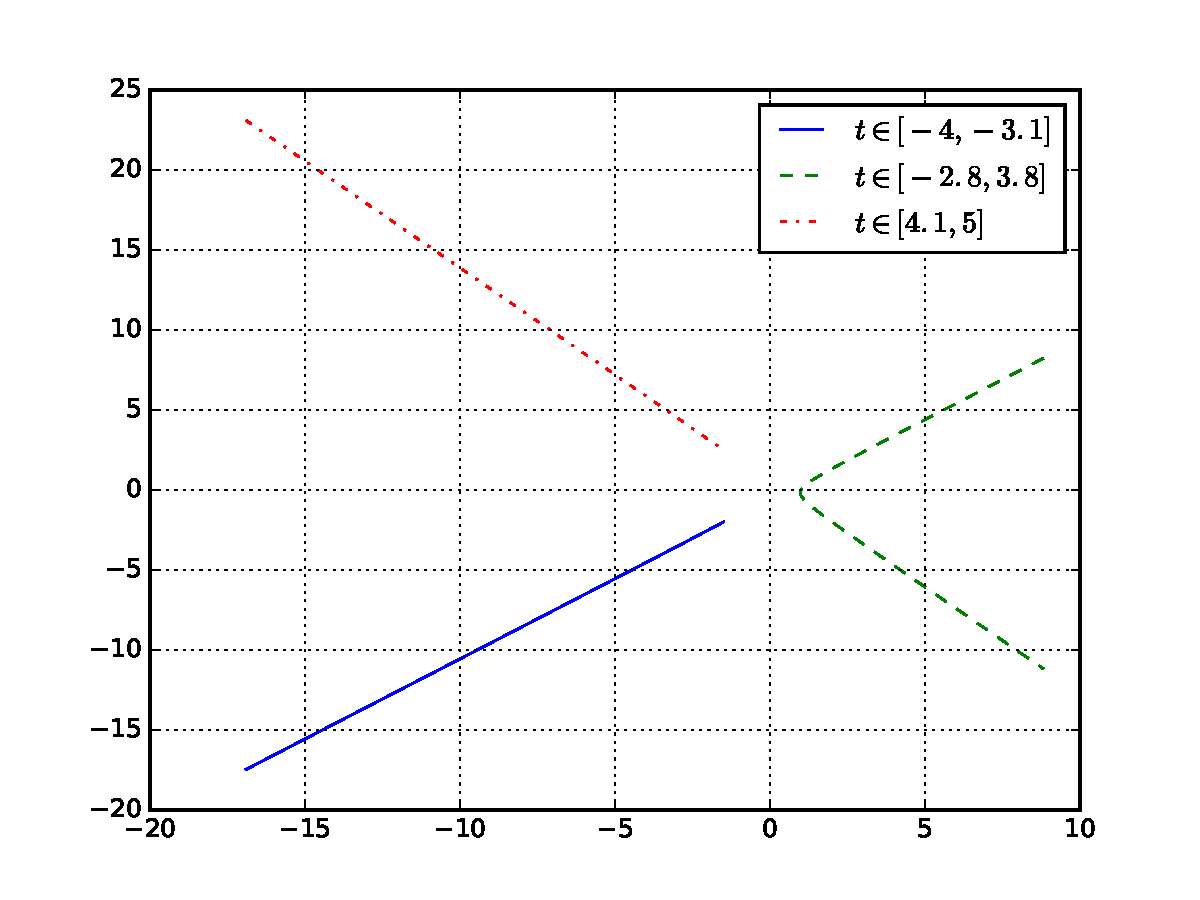
\includegraphics[width=\textwidth]{graphe.pdf}

Le code, en {\sffamily Python} :

\lstset{basicstyle=\ttfamily,language={Python},numbers=left, numberstyle=\tiny, numbersep=5pt}
\begin{lstlisting}
import numpy as np
import matplotlib
import matplotlib.pyplot as plt

def F(t):
    a = t*t - t - 12
    return (-12/a,4*t/a)

bounds = [[-4,-3.1],[-2.8,3.8],[4.1,5]]
opt = ['-','--','-.']
fig = plt.figure()
ax = fig.add_subplot(111)
for i, b in enumerate(bounds):
    T = np.linspace(*b,300)
    X,Y = F(T)
    lbl = r'$t\in[{0}, {1}]$'.format(b[0],b[1])
    ax.plot(X,Y, opt[i],label=lbl)

ax.legend()
ax.grid()
fig.show()
\end{lstlisting}

\end{document}